% !TeX root = main.tex
\documentclass[conference]{IEEEtran}
\IEEEoverridecommandlockouts
% The preceding line is only needed to identify funding in the first footnote. If that is unneeded, please comment it out.
\usepackage{cite}
\usepackage{amsmath,amssymb,amsfonts}
\usepackage{algorithmic}
\usepackage{graphicx}
\usepackage{textcomp}
\usepackage{xcolor}
\usepackage{subfiles}
\graphicspath{{\subfix{images/}}}

\def\BibTeX{{\rm B\kern-.05em{\sc i\kern-.025em b}\kern-.08em
    T\kern-.1667em\lower.7ex\hbox{E}\kern-.125emX}}
\begin{document}

\title{
	Supervised Neural Network Training\\
	{\footnotesize COS 711 - Assignment 2}
}

\author{\IEEEauthorblockN{1\textsuperscript{st} Ushir Raval}
\textit{u16013604} \\
u16013604@tuks.co.za
}

\maketitle

\begin{abstract}
The purpose of this report is to demonstrate the performance implications of Passive training methods with a focus on Simple Gradient Decent and Newtonian Gradient Methods (specifically Conjugate Gradient Decent) in contrast with Curriculum Learning. The findings from the variuous documented experiments, using the Sloan Digital Sky Survay data, indicate that while both Curriculum Learning and 'Augmented' Passive learning display subtle improvements to the ratio of Neural Network Accuracy vs Training 'Costs', Curriculum Learning may be a more robust solution despite being more prone to erroneous implementation.
\end{abstract}

\section{Introduction}
In Neural Network Optimization, most academics have moved on to more novel methods such as Deep Neural Nets and Cascading Networks. However, some techniques can be used to optimise more basic Simple Neural Networks that fall in line with Occums Razor \cite{supervised-learning-slides}.
Using novel methods such as Curriculum Learning or more mathematically complex optimizations like Newton's methods provide simple networks with very high accuracies. As demonstrated in this report, both Methods sufficiently optimise Neural Networks to 'production' level accuracies while being relatively cheap to compute which small training times.


\section{Background}
In order to determine objects from a Dataset of data constructed from multiple domains, a Neural Network was used as a Classifier. 
This produced an optimal test case to compare two techniques used for improving Supervised Learning, altering the gradient decent algorithm contrasted with altering the training method of the network.
Both of these methods produce fairly good improvements over our baseline, what we will call a 'Simple' Network for the scope of this report, will define a network using the standard Stochastic Gradient Decent \cite{ketkar2017stochastic} (without momentum) with a standard consistent size batch training optimizer.

\subsection{Conjugate Gradient Method}
Newton's Method for reaching the optimal valley of an set of equations in X-dimensions requires the costly computation of a Hessian Matrix to encode the information of the curvature. This is then used in the calculation of the optimal (X-1)-dimensional plane within the search space which the optimizer may use to effectively map a path to a better solution from the current point in the search space.\cite{supervised-learning-slides}
\\\\
The Conjugate Gradient Method is essentially a better architected implementation of Newton's Method which uses a conjugate gradient\cite{supervised-learning-slides} to do a number of steps from the normal Newton's Method in a single jump. This provides two benefits:
\begin{itemize}
	\item Allows us to ensure that we do not revert any optimizations/jumps previously done
	\item Uses a linear method which is more efficient then the Hessian updates needed for normal Newton Methods
\end{itemize}
This means while we get largely similar results when compared to a straight forward Newton's Method, we converge with much less iterations.
\\\\
The known problems with Conjugate Gradient Decent are mostly to do with the same computational difficulties that arise with Ordinary Newton's Method where the adjustments provide a significant overhead since they are approximated quadratically.

\subsection{Curriculum Learning Method}

This Method calls for the novel use of one Pre-trained Simple Network (hereby called the 'Inception' Network) training a production network from it's output.
This is in accordance with the Curriculum Learning algorithm described in \cite{on-the-power}. Where a figurative 'professor' determines the curriculum before the training of the 'production' network by training a 'development' (or inception) network and using it to grade the input dataset into levels of difficulty.
The dataset is then split by order of its simplicity and used to train the production network in batches while incrementally adding harder 'problem sets' to the 'curriculum'.
\\
This Method does well to minimize overfitting and increases accuracy at the cost of training time and more complex data preparation methods.

\section{Experimental Set-Up}

\subsection{Data Preparation}
Upon analysis of the Sloan Dataset, the data was found to be lacking for the purposes of a Neural Network, therefore a number of operations where performed in the preprocessing stage documented as follows.
\\
\textbf{Removing Obviously Irrelavent Inputs}\\
a. Removing Obviously Irrelavent Inputs:
Our dataset is basically made up of 4 sections:
\begin{enumerate}
	\item Position of Object in Space
	\item Magnitude of Object
	\item Image Metadata
	\item Spectral Readings
\end{enumerate}
Since our NN's will be used to predict \textit{astronomical objects} based on recorded \textit{physical} observations, section 3 is not needed, but as positions of objects could be an indicator of what they are in the context of relativity to another celestial body. For example, an object's likelihood of being a planet goes up if it is orbiting a star. As such, the fields ra, dec, u, g, r, i, z from the Object position and Thaum-Guan magnitude system as well as the redshift from the Spectral Readings will be used to determine the object class, which is a discrete set which consists of Galaxy, Quasar and Star.
\\
\textbf{Encoding Categorical Data}
\\
The output column 'class' is a discrete set which consists of Galaxy, Quasar and Star. As such Binary One-Hot Encoding was used to convert this to a numerical feature.
\\
\textbf{Normalisation and Scaling}
\\
\begin{figure}[h]
	\caption{Distribution of Raw Dataset}
	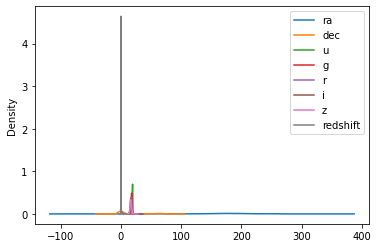
\includegraphics[scale=0.5]{raw-distribution}
	\centering
	\label{fig:dist-raw}
\end{figure}

\begin{figure}[h]
	\caption{Distribution of Normalized Dataset}
	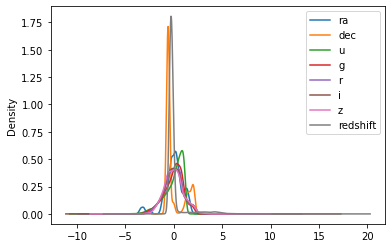
\includegraphics[scale=0.5]{normalised-data-dist}
	\centering
	\label{fig:dist-normed}
\end{figure}
Looking at the distribution graph of the dataset in figure \ref{fig:dist-raw} We see that the ranges between the columns are significantly different, therefore, using mean normalization with the formula:
\begin{equation}
	Z^{MV}_{i,p} = \frac{Z_{i,p}-\bar{Z_i}}{\sigma_{Z_i}}
\end{equation}

We get figure \ref{fig:dist-normed}.

\subsection{Simple Neural Network}
In order to compare the novel methods a baseline Simple Neural Network was created with choice hyper-parameters optimised as below. The network had an input layer of 8 with 2 hidden layers of 9 nodes each with 'relu' activation and 1 output layer of 3 nodes with 'sigmoid' activation.
\subsubsection{Number of Layers}
The choice of number of layers of a Neural Network is largely determined by 'how much' the dataset is 'linearly separable' into it's respective classes. The general 'rule of thumb' is that your number of layers should be larger then one when there is at least one correlation distribution that displays non-separable clustering. \cite{s-j-kwon-anns}
As such, an observational method was used where a scatter matrix was generated to determine visually if various parameter correlations could be grouped. This 'visual' method was deemed to be sufficient as clustering was clearly visible in some variables.
\begin{figure}
	\caption{Scatter Matrix Plot to show Clustering of Features in correlation with each other}
	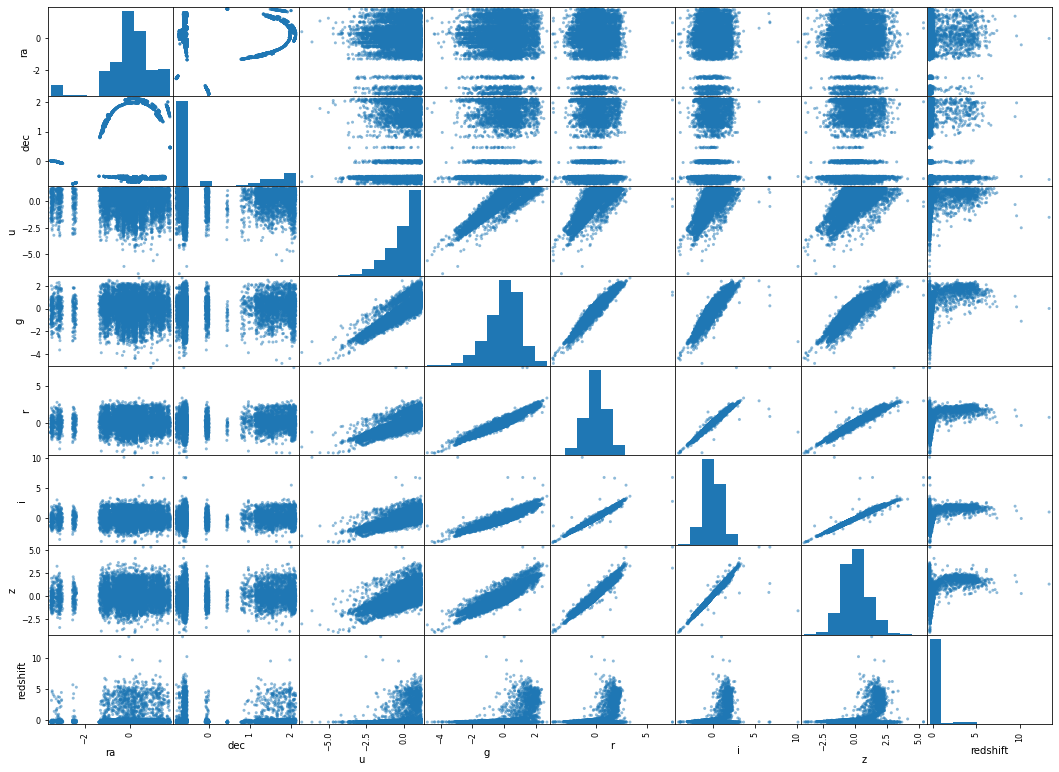
\includegraphics[width=0.5\textwidth]{scatter-mat}
	\centering
	\label{fig:scatter-matrix}
\end{figure}

We can see in figure \ref{fig:scatter-matrix} that features such as 'u' and 'redshift' do not display any visible clustering patterns and as such a single layer ANN would not be expected as an optimal solution.
The number of layers was decided to be two as adding more displayed no signs of improvement during training. Less then two layers was shown to produce erroneous results with a very lossy ANN.

\subsubsection{Number of Hidden Nodes}
The number of hidden nodes was chosen to be 9 initially, which provided considerable improvement over 8 (below which the results where comparatively poor). Increasing the number of nodes beyond 9 shows no observable signs of improvement with accuracy however performed fractionally faster. 
Due to the complex nature of the following Experiments, 9 was thought to be sufficiently performant while keeping complexity lower.

\subsubsection{Activation Functions}
Since the output of the Neural Network is a vector of size 3 with data points within range 0 and 1, the Softmax Activation function was chosen. Additionally an extra step of data-preprocessing was done to scale the one-hot encoded outputs to have a minimum of 0.1 instead of 0 and 0.9 instead of 1 in order to more accurately assess loss in the network.
The Sigmoid Activation function was shown to have similar results with respect to accuracy but was slightly more lossy (please see Appendix A for comparison).

\subsubsection{Optimisation Algorithm Parameters}
The Stochastic gradient decent Optimizer was used with a Batch Size of 30 with 50 epochs. Smaller Batch Sizes converged more slowly per epoch but in less iterations (please see Appendix A for results).

\subsection{Conjugate Gradient Neural Network}
The Conjugate Gradient Neural Network used the same hyper-parameters as the Simple Network above, however a Custom Optimizer was created that performed a standard conjugate gradient adjustment instead of the Stochastic Gradient Adjustments done above.

\subsection{Curriculum Learning Neural Network}
As with the Conjugate Gradient Network, this used the same hyper-parameters as the Simple Network, however two instances of the network were used. As such there are a few additional hyper-parameters added, namely:
\subsubsection{Scoring Function}
Chosen for it's relative simplicity, the Self-taught Scoring function was used as it fit into the experimental set-up with the least disruption. A 'development' network was already prepared in the form of the Simple Network described above.

\subsubsection{Pacing Function}
This function is used to determine the size of the increments added to the 'curriculum'. The Fixed Exponential Pacing was chosen due to it's simplicity.

\begin{equation}
	g_v(i) = min(starting percent\times inc^{\frac{i}{step length}})\times N
\end{equation}

\subsubsection{Starting Percent}
Using in the Pacing function, the starting percent has a large impact on the training time as well as the model convergence. A smaller starting step displayed a longer convergence time to a slightly lower average accuracy while the corollary was also proven to be true. This was chosen to be 50\% of the training dataset largely to have optimal training times.

\subsubsection{Increment}
The $inc$ in the Pacing function determines the increment size and a smaller value naturally increases the training time. Care must be taken to not have the pacing function display an asymptote that appears before the end of the dataset as this will lead to an infinite training loop in the 'Curriculum' Algorithm. An 'inc' value of 0.2 was found to have the best optimization vs convergence time ratio

\section{Research Results}
\subsection{Simple Network Results}
\begin{figure}
	\caption{Graph to show the mean General Accuracy over 5 independently trained neural networks}
	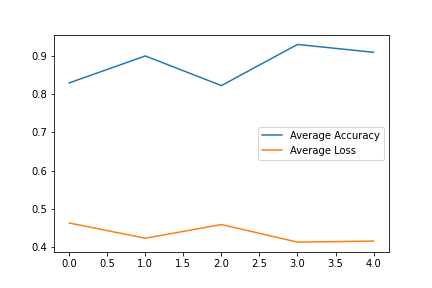
\includegraphics[width=0.5\textwidth]{eval-mean-performace}
	\centering
	\label{fig:eval-mean}
\end{figure}

\begin{figure}
	\caption{Graph to show the Average Training Accuracy vs Validation Accuracy}
	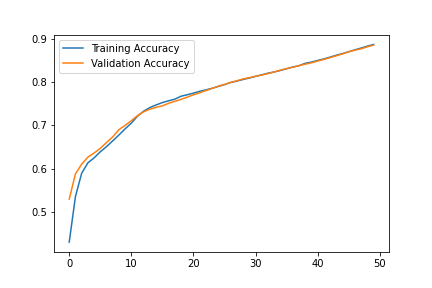
\includegraphics[width=0.5\textwidth]{mean-accuracy}
	\centering
	\label{fig:mean-acc}
\end{figure}

\begin{figure}
	\caption{Graph to show the Average Standard Deviation During Training}
	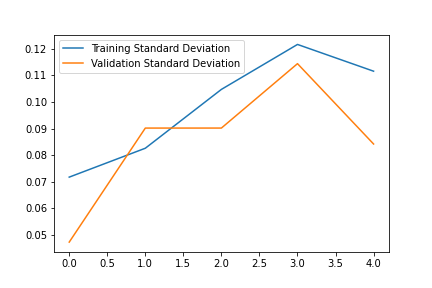
\includegraphics[width=0.5\textwidth]{mean-std}
	\centering
	\label{fig:mean-std}
\end{figure}

Being a fairly straight-forward ANN, the Simple Network had a fairly good max average optimization of approximately 93\% with a loss of on average 37\% and converging in approximately 30 seconds per training session.
This was to be expected as the Input data was well normalized and fairly suited to a Neural Network Classifier with an Extra layer to handle variables that were not clustered well.

Adding more hidden nodes per layer produced no significant difference in accuracy or loss, however adding more layers, while not producing any statistically relevant improvements to the mean accuracy, had a significantly lower loss that averaged at approximately 20\%. However this resulted in approximately 50\% longer time to convergence and thus was excluded due to the additional overheads produced by the Conjugate Gradient Network and the Curriculum Network.

\subsection{Conjugate Gradient Decent}

\begin{figure}
	\caption{Graph to show the Average Training Accuracy vs Validation Accuracy}
	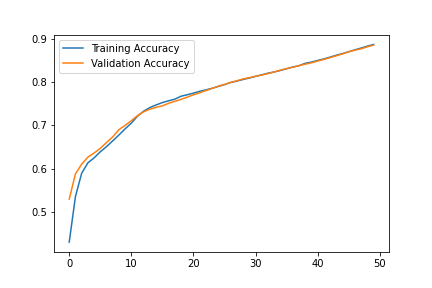
\includegraphics[width=0.5\textwidth]{mean-accuracy}
	\centering
	\label{fig:mean-acc-c}
\end{figure}

\begin{figure}
	\caption{Graph to show the Average Standard Deviation During Training}
	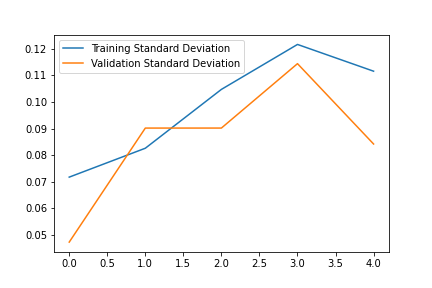
\includegraphics[width=0.5\textwidth]{mean-std}
	\centering
	\label{fig:mean-std-c}
\end{figure}

As seen in figure \ref{fig:mean-acc-c}, the conjugate gradient decent provides slightly better accuracies and losses averaging at approximately 95\% accuracy and 34\% loss with a much smaller number of Epochs required. However, a single run took significantly longer with an average of 30 seconds per run totaling at 15 mins per training session of 50 epochs.

\subsection{Curriculum Learning}

\begin{figure}
	\caption{Graph to show the Average Training vs Validation Accuracy on Parameter Set 1}
	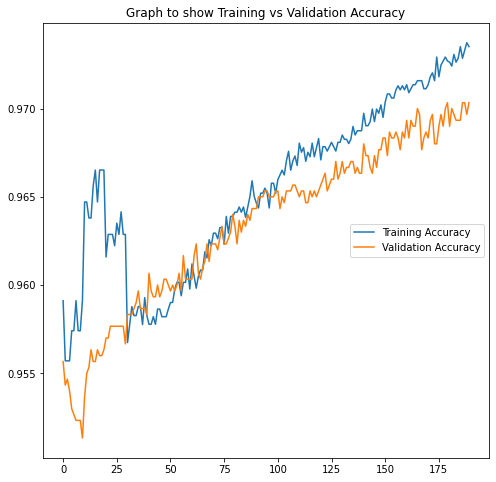
\includegraphics[width=0.5\textwidth]{cl-train-vs-val}
	\centering
	\label{fig:cl-set-1}
\end{figure}

\begin{figure}
	\caption{Graph to show the Average Training vs Validation Accuracy on Parameter Set 1}
	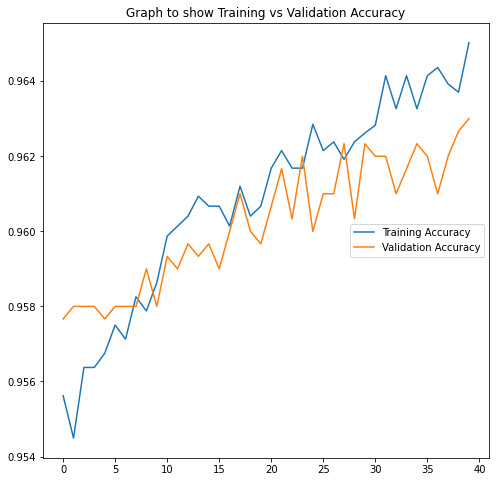
\includegraphics[width=0.5\textwidth]{cl-train-vs-val-pramset2}
	\centering
	\label{fig:cl-set-2}
\end{figure}

\begin{figure}
	\caption{Graph to show the Average Training vs Validation Accuracy on Parameter Set 1}
	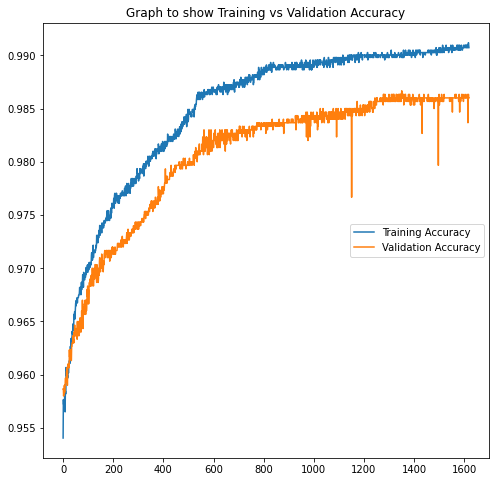
\includegraphics[width=0.5\textwidth]{cl-train-vs-val-paramset3}
	\centering
	\label{fig:cl-set-2}
\end{figure}

With Curriculum Learning the figure \ref{fig:cl-set-1} had the most optimal network when time to convergence was considered had the following hyper-parameters:
\begin{itemize}
	\item Starting percent = 0.6
	\item Increasing data size = 0.3
	\item Step length = 10
\end{itemize}

This NN converged at an average accuracy of 98.20\% with an average loss of 37.20\% taking 2 mins to converge.

We can see that in figure \ref{fig:cl-set-2} with the hyper-parameters:
\begin{itemize}
	\item Starting Percent = 0.5
	\item Increment = 0.2
	\item Step Length = 10
\end{itemize}

While this parameter set resulted in a faster convergence to parameter set 1, we can see massive jump when the initial batch is used to train the NN with 'easy examples' and a noticeable dip in accuracy as the problems become 'harder'. This NN converged at an average accuracy of 96.20\% with a loss of 37\% taking approximately 1 minute.

The NN with the longest convergence time can be seen in figure \ref{fig:cl-set-3} with eh following hyper-parameters:
\begin{itemize}
	\item Starting Percent = 0.6
	\item Increment = 0.3
	\item Step Length = 4
\end{itemize}

This also had an extremely high average accuracy of 99\% and a loss of 33\%, however this took approximately 10 mins to converge, nearly 500\% longer then the next most optimal solution.




\section{Conclusion}

The novel methods discussed in this paper prove to have significant results on Networks with significant differences in approaches.
On average the curriculum learning provided the most positive impact on a Simple Neural Network and far surpasses the results of the baseline model. However the concern raised earlier in the report stands. The Curriculum learning method is the most prone to user error as the preprocessing of the data provides ample opportunity to create false correlations (for example, if scored incorrectly). 
Conjugate gradient decent, while simple to implement in comparison, provides little improvement with higher cost w.r.t. time to convergence for training.
These trade-offs prove that Curriculum Learning has a statistical 'edge' over Conjugate Gradient as well as providing a highly optimal Classifier. This proves that data preprocessing has profound effects on training and Optimizations that potentially surpass the importance of a novel decent algorithm or path finder.

\section{Appendix A}

\subsection{Sigmoid vs Softmax Activation functions}
x
\subsection{Batch Size vs Number of Epochs}
y


\bibliographystyle{IEEEtran}
\bibliography{refs}

\vspace{12pt}
\color{red}

\end{document}
